\documentclass{article}
\usepackage[LGR, T1]{fontenc}
\usepackage[greek]{babel}
\usepackage{cancel}
\usepackage{amsmath}
\usepackage{tikz}
\usetikzlibrary{trees}
\begin{document}
\title{\textlatin{question1}}
\maketitle
\section*{ΕΚΦΩΝΗΣΗ:}

\subsection*{Πρόβλημα 1}
Αποδείξτε τον εξής ισχυρισμό. Για κάθε δένδρο παιχνιδιού, η χρησιμότητα για τον \textlatin{MAX} που
υπολογίζεται χρησιμοποιώντας αποφάσεις \textlatin{minimax} εναντίον ενός μη βέλτιστου (\textlatin{suboptimal}) \textlatin{MIN} δεν
είναι ποτέ μικρότερη από την χρησιμότητα που υπολογίζεται παίζοντας εναντίον ενός βέλτιστου \textlatin{MIN}.
Μπορείτε να βρείτε ένα δένδρο παιχνιδιού στο οποίο ο \textlatin{MAX} μπορεί να τα καταφέρει ακόμα καλύτερα
χρησιμοποιώντας μια μη βέλτιστη (\textlatin{suboptimal}) στρατηγική εναντίον ενός μη βέλτιστου \textlatin{MIN}?


\section*{ΑΠΑΝΤΗΣΗ:}

Θα αποδείξουμε τον ισχυρισμό με απαγωγή σε άτοπο. Οι υποθέσεις είναι ότι ο \textlatin{MAX} παίζει βέλτιστα, ενώ ο \textlatin{MIN} δεν παίζει βέλτιστα, και έστω ότι η χρησιμότητα για τον \textlatin{MAX} είναι μικρότερη από αυτήν που θα είχε εναντίον έναν βελτιστο \textlatin{MIN}.
\\ \\
Εφ'όσον και στις δύο περιπτώσεις ο \textlatin{MAX} παίζει βέλτιστα, οποιαδήποτε διαφοροποίηση στην χρησιμότητα θα προέρχεται από αλλαγή στις κινήσεις του \textlatin{MIN}. Με άλλα λόγια, υπονοούμε ότι ο μη βέλτιστος \textlatin{MIN} πρέπει να έχει κάνει τουλάχιστον μία επιλογή που οδήγησε σε χαμηλότερη χρησιμότητα για τον \textlatin{MAX} από ό,τι θα επέλεγε o βέλτιστος \textlatin{MIN}. Άτοπο, διότι ο βέλτιστος \textlatin{MIN} πάντα ελαχιστοποιεί την χρησιμότητα του \textlatin{MAX}.
Άρα η αρχική μας υπόθεση είναι λάθος, άρα ο ισχυρισμός είναι αληθής.
\\ \\
Όσο για το δέυτερο ερώτημα, ας εξετάσουμε αυτό το δέντρο:

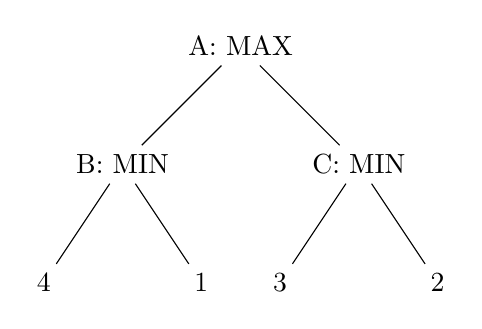
\begin{tikzpicture}[
    level distance=1.5cm,
    level 1/.style={sibling distance=3cm},
    level 2/.style={sibling distance=2cm}
]
\node {\textlatin{A}: \textlatin{MAX}}
    child {
        node {\textlatin{B}: \textlatin{MIN}} 
        child {
            node {4}
        }
        child {
            node {1}
        }
    }
    child {
        node {\textlatin{C}: \textlatin{MIN}}
        child {
            node {3}
        }
        child {
            node {2}
        }
    };
\end{tikzpicture}
\\ \\


Σε αυτό το δέντρο: \\ \\
Χρησιμοποιώντας το βέλτιστο \textlatin{minimax}: \\
Στον κόμβο \textlatin{B}, ο \textlatin{MIN} θα επέλεγε 1 \\
Στον κόμβο \textlatin{C}, ο \textlatin{MIN} θα επέλεγε το 2 \\
Στον κόμβο \textlatin{A}, ο \textlatin{MAX} θα επέλεγε το \textlatin{C}, λαμβάνοντας χρησιμότητα 2 \\
\\ \\
Τώρα ας υποθέσουμε: \\
Ο \textlatin{MAX} παίζει μη βέλτιστα και επιλέγει B \\
Ο \textlatin{MIN} παίζει μη βέλτιστα και επιλέγει το 4 στο B \\
Εδώ, ο \textlatin{MAX} παίρνει χρησιμότητα 4 παίζοντας μη βέλτιστα εναντίον ενός μη βέλτιστου \textlatin{MIN}, μεγαλύτερη από αυτή που θα είχε πάρει αν έπαιζε βέλτιστα. \\

\end{document}
